\documentclass{article}

\usepackage[final]{nips}

\usepackage[utf8]{inputenc} % allow utf-8 input
\usepackage[T1]{fontenc}    % use 8-bit T1 fonts
\usepackage{hyperref}       % hyperlinks
\usepackage{url}            % simple URL typesetting
\usepackage{booktabs}       % professional-quality tables
\usepackage{amsfonts}       % blackboard math symbols
\usepackage{nicefrac}       % compact symbols for 1/2, etc.
%\usepackage{microtype}      % microtypography
\usepackage{amsmath}
\usepackage{bm}
\usepackage{tikz}
\usepackage{graphicx}
\usepackage{subcaption}
\usepackage{float}
\usetikzlibrary{bayesnet}
\graphicspath{ {images/} }

\newcounter{question}
\newcommand{\question}{\stepcounter{question}\paragraph{Question \thequestion}}
\newcommand{\mat}[1]{\textbf{\textit{#1}}}
\DeclareMathOperator{\Tr}{Tr}
\DeclareMathOperator{\argmin}{arg\,min}
\DeclareMathOperator{\argmax}{arg\,max}

\title{Coursework 1 - Modelling}

\author{
  Jonas Osborn \\
  \texttt{jo14944} \\
  \And
  Tristan Saunders \\
  \texttt{ts16802} \\
  \And
  Corin Varney \\
  \texttt{cv14985} \\
}

\begin{document}

\maketitle

\section{The prior}
\subsection{Theory}
\question \emph{1.} Choosing a gaussian is a sensible thing to do because it makes calculation much easier, Gaussians are quite easily multiplied and integrated which are things you often have to do in machine learning contexts e.g. multiplying to compute a joint distribution or integrating to marginalise out a variable. Choosing a Gaussian likelihood is also sensible as it fits with our model because we often assume observation errors to be independent and identically distributed and therefore Gaussian due to the Central Limit Theorem.

\emph{2.} Choosing a spherical covariance matrix for the likelihood means that we are assuming the different dimensions of $y_i$ to be independent and identically distributed. As they are independent they do not covary with each other and so the covariance matrix is diagonal. As they are identically distributed they all have the same variance. Therefore the covariance matrix is spherical.
\question
\begin{align*}
	p(\mat{Y}|f,\mat{X}) &= p(y_1,\ldots,y_{N-1},y_N|f,\mat{X}) \\
	&= p(y_N|y_{N-1},\ldots,y_1,f,\mat{X})p(y_{N-1}|y_{N-2},\ldots,y_1,f,\mat{X})\ldots p(y_1|f,\mat{X}) \\
\end{align*}
\subsubsection{Linear regression}
\question We assume that the data is independent and so the joint probability is a product.
\begin{align*}
	p(\mat{Y}|\mat{X},\mat{W}) &= \prod_{i}^Np(\mat{y}_i|\mat{x}_i,\mat{W}) \\
	&= \prod_{i}^N\mathcal{N}(\mat{W}\mat{x}_i,\sigma^2\mat{I}) \\
\end{align*}
\question A conjugate prior is one that is conjugate to the posterior, meaning they are in the same family of distributions. A conjugate prior is useful as it gives a closed-form solution for the posterior. If we didn't choose a conjugate prior then numerical integration may be necessary to calculate the posterior, which may mean the solution is potentially intractable. The conjugate prior for a Gaussian posterior is a Gaussian.
\question Just as encoding the prefrence in a $L_2$ norm is equivalent to having a Gaussian prior, encoding the preference using a $L_1$ norm is equivalent to having a Laplace prior. This is because the Laplace distribution estimates median rather than the mean estimated by the Guassian and median minimises the $L_1$ norm and mean the $L_2$.

The shape of the laplace distribution's probability density function, with it's higher peak around zero compared to the probability density function of a Gaussian means that more co-efficients are likely to be equal to zero and this leads to a sparser model than those produced by a Gaussian prior.
\question
\begin{align*}
	p(\mat{W}|\mat{X},\mat{Y}) &= \frac{1}{Z}p(\mat{Y}|\mat{X},\mat{W})p(\mat{W}) \\
	&= \frac{1}{Z}\mathcal{N}(\mat{W}\mat{X},\sigma^2\mat{I})\mathcal{N}(\mat{W}_0,\tau^2\mat{I})
\end{align*}
$\frac{1}{Z}$ is the normalising constant to ensure that the posterior is a probability density function by making the area under the graph equal to $1$, this constant is called the evidence. We will ignore it for now.

By the probability density function of the multivariate normal distribution, we have:
\begin{align*}
	p(\mat{W}|\mat{X},\mat{Y}) \propto\ &\frac{1}{\sqrt{(2\pi)^N\sigma^2}}\exp\bigg(-\frac{1}{2\sigma^2}(\mat{Y}-\mat{X}\mat{W})^T(\mat{Y}-\mat{X}\mat{W})\bigg) \\
	&\cdot \frac{1}{\sqrt{(2\pi)^N\tau^2}}\exp\bigg(-\frac{1}{2\tau^2}(\mat{W}-\mat{W}_0)^T(\mat{W}-\mat{W}_0)\bigg) \\
\end{align*}
We ignore the normalising constants as we re-normalise with $Z$ and then combine and multiply out the exponents.
\begin{align*}
	p(\mat{W}|\mat{X},\mat{Y}) \propto\ &\exp\bigg(-\frac{1}{2\sigma^2}(\mat{Y}-\mat{X}\mat{W})^T(\mat{Y}-\mat{X}\mat{W})-\frac{1}{2\tau^2}(\mat{W}-\mat{W}_0)^T(\mat{W}-\mat{W}_0)\bigg) \\
	\propto\ &\exp\bigg(-\frac{1}{2\sigma^2}(\mat{Y}^T\mat{Y}-2\mat{Y}^T\mat{X}\mat{W}+\mat{W}^T\mat{X}^T\mat{X}\mat{W}) \\
	&\hspace{2.5em}-\frac{1}{2\tau^2}(\mat{W}_0^T\mat{W}_0-2\mat{W}^T\mat{W}_0+\mat{W}^T\mat{W})\bigg)
\end{align*}
We know the posterior will be Gaussian as both the likelihood and prior are, so we can assume it will take the form: $\exp\big((\mat{W}-\mu)^T\mathbf{\Sigma}^{-1}(\mat{W}-\mu)\big)$. If we multiply the exponent out we get a quadratic so we try and make the posterior we have look like this quadratic.
\begin{align*}
	p(\mat{W}|\mat{X},\mat{Y}) \propto \exp\bigg(&-\frac{1}{2\sigma^2}\mat{W}^T\mat{X}^T\mat{X}\mat{W}-\frac{1}{2\tau^2}\mat{W}^T\mat{W}	&&\mbox{quadratic term}\\
	&+\frac{1}{\sigma^2}\mat{W}^T\mat{X}^T\mat{Y}+\frac{1}{\tau^2}\mat{W}^T\mat{W}_0							&&\mbox{mixed term}\\
	&-\frac{1}{2\sigma^2}\mat{Y}^T\mat{Y}-\frac{1}{2\tau^2}\mat{W}_0^T\mat{W}_0\bigg)							&&\mbox{constant term}\\
\end{align*}
By re-arranging and completing the square we can find both $\mathbf{\Sigma}^{-1}$ and $\mathbf{\Sigma}^{-1}\mu$ in the quadratic and mixed terms respectively.
\begin{align*}
	p(\mat{W}|\mat{X},\mat{Y}) \propto \exp\bigg(&-\frac{1}{2}\mat{W}^T\overbrace{\Big(\frac{1}{\sigma^2}\mat{X}^T\mat{Y}+\frac{1}{\tau^2}\mat{I}\Big)}^{\mathbf{\Sigma}^{-1}}\mat{W}	&&\mbox{quadratic term}\\
	&+\mat{W}^T\underbrace{\Big(\frac{1}{\sigma^2}\mat{X}^T\mat{Y}+\frac{1}{\tau^2}\mat{W}_0\Big)}_{\mathbf{\Sigma}^{-1}\mu}						&&\mbox{mixed term}\\
	&-\frac{1}{2\sigma^2}\mat{Y}^T\mat{Y}-\frac{1}{2\tau^2}\mat{W}_0^T\mat{W}_0\Big)								&&\mbox{constant term}\\
\end{align*}
From these we can easily find $\mathbf{\Sigma}$ and $\mu$.
\begin{align*}
	\mathbf{\Sigma} = &\bigg(\frac{1}{\sigma^2}\mat{X}^T\mat{Y}+\frac{1}{\tau^2}\mat{I}\bigg)^{-1} \\
	\mathbf{\Sigma}^{-1}\mu = &\frac{1}{\sigma^2}\mat{X}^T\mat{Y} + \frac{1}{\tau^2}\mat{W}_0 \\
	\mu = &\mathbf{\Sigma}\bigg(\frac{1}{\sigma^2}\mat{X}^T\mat{Y} + \frac{1}{\tau^2}\mat{W}_0\bigg) \\
\end{align*}
Thus we have our posterior as a Guassian with our values for $\mathbf{\Sigma}$ and $\mu$:
\begin{align*}
	p(\mat{W}|\mat{X},\mat{Y}) \propto\ &\exp\bigg(-\frac{1}{2}(\mat{W}-\mu)^T\Sigma^{-1}(\mat{W}-\mu)\bigg)\\
	\propto\ &\mathcal{N}\bigg[\Big(\frac{1}{\sigma^2}\mat{X}^T\mat{Y}+\frac{1}{\tau^2}\mat{I}\Big)^{-1}\Big(\frac{1}{\sigma^2}\mat{X}^T\mat{Y} + \frac{1}{\tau^2}\mat{W}_0\Big),\Big(\frac{1}{\sigma^2}\mat{X}^T\mat{Y}+\frac{1}{\tau^2}\mat{I}\Big)^{-1}\bigg]
\end{align*}
\subsubsection{Non-parametric regression}
\question Parametric models assume that the distribution the data comes from is based on a finite, fixed set of parameters and models future predictions based off these parameters, they capture everything there is to know about the data. Non-parametric models do not make such assumptions about the model structure and instead infer structure from the data, they have parameters but these are not fixed in advance and there can be an infinite set of parameters.

Non-parametric models are more flexible and can represent a wider variety of data and will represent the data better if the assumptions made in the parametric model are incorrect but are less precise and accurate than parametric methods if the right assumptions are made.

Parametric models are often easier interpreted as they are simpler to transcribe and are also often faster to compute due to lacking the complexity and flexibility of the non-parametric models.
\question As we use a Gaussian process we define this prior over functions and want our prior to put some constraints on the space of functions. The fact that its a Gaussian process means that for an arbitary set of points $x_i, \ldots, x_j$ we assume that $p(f_i), \ldots,f(x_j))$ is jointly Gaussian with mean $0$ and covariance function $k$, from this we have the equation for our prior:
$$
	p(f|\mat{X},\bm{\theta}) = \mathcal{N}(0, k(\mat{X},\mat{X}))
$$
The covariance function $k$ allows us to set constraints from our assumptions about the mapping $f$. For example, our assumption about the functions smoothness that if $x_i$ and $x_j$ are similar then we expect $f_i$ and $f_j$ to be similar too, with certain kernel functions for $f$ we can only sample functions that have sufficient smoothness by ensuring that constraint.
\question Gaussian processes encode all possible functions for which inferring a posterior distribution from the data is tractable.
\question
\begin{align*}
	p(\mat{Y},\mat{X},f,\bm{\theta}) = p(\mat{Y}|f)p(f|\mat{X},\bm{\theta})p(\mat{X})p(\bm{\theta})
\end{align*}
\begin{center}
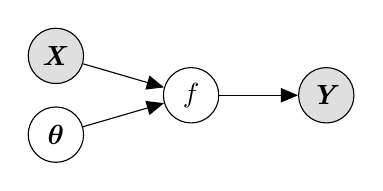
\begin{tikzpicture}
	\node[obs] (Y) {$\mat{Y}$}; %
	\node[latent, left=of Y] (f) {$f$} ; %
	\node[obs, left=of f, yshift=0.5cm] (X) {$\mat{X}$} ; %
	\node[latent, left=of f, yshift=-0.5cm] (theta) {$\bm{\theta}$} ; %
	\edge {X,theta} {f}; %
	\edge {f} {Y}; %
\end{tikzpicture}
\end{center}
\begin{itemize}
	\item $\mat{X}$ and $\bm{\theta}$ are independent
	\item $f$ is conditionally dependent on both $\mat{X}$ and $\bm{\theta}$
	\item $\mat{Y}$ is conditionally dependent on $f$ and conditionally independent of $\mat{X}$ and $\bm{\theta}$
\end{itemize}
\question This marginalization shows the likelihood of the data we have observed over the function we are testing which is constrained by the prior.

There are two sources of uncertainty here, that associated with $f$ in the prior and that associated with $\epsilon$ in the likelihood, these are independent and as such are merged by simply adding to form the covariance of the marginal likelihood Gaussian.

Leaving the $\theta$ on the left-hand side of the expression implies that we still have specific hyperparameters rather than undefined ones. It remains throughout the integral.
\subsection{Practical}
\subsubsection{Linear regression}
\question Figure \ref{fig:prior} represents our prior assumption over $\mat{W}$. Our prior assumption states that the distribution over $\mat{W}$ is a Gaussian with a mean of $0$ and the identity matrix as its covariance. As discussed in question 3 the likelihood is a Gaussian, therefore choosing a Gaussian prior allows us to obtain a Gaussian posterior.

In Figures \ref{fig:1-s}, \ref{fig:2-s} and \ref{fig:15-s} we can see how our assumptions about $\mat{W}$ change as we observe more data. Making the distribution over $\mat{W}$ a posterior or our updated belief. These are paired with samples from our posterior that allow us to plot some sample functions. It is clear that the more data we observe, the more the uncertainty in our posterior reduces, giving us a posterior that approaches the exact values of the actual parameters $\mat{W}$ (displayed as a white cross) along with increasingly accurate sample functions.
\begin{figure}[H]
	\centering
	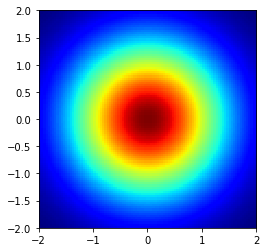
\includegraphics[width=0.3\linewidth]{prior}
	\caption{Prior for linear regression}
	\label{fig:prior}
\end{figure}
\begin{figure}[H]
	\centering
	\begin{subfigure}[t]{0.3\linewidth}
		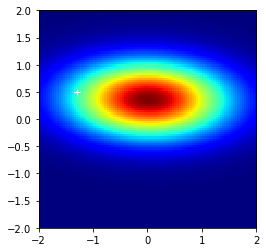
\includegraphics[width=\linewidth]{1-posterior}
		\caption{Posterior}
		\label{fig:1-p}
	\end{subfigure}
	\begin{subfigure}[t]{0.3\linewidth}
		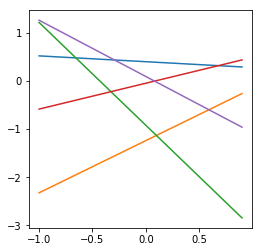
\includegraphics[width=\linewidth]{1-samples}
		\caption{Samples of $y$}
		\label{fig:1-s}
	\end{subfigure}
	\caption{Linear regression - 1 observation}
	\label{fig:1-s}
\end{figure}
\begin{figure}[H]
	\centering
	\begin{subfigure}[t]{0.3\linewidth}
		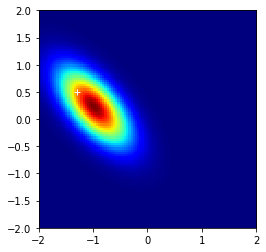
\includegraphics[width=\linewidth]{2-posterior}
		\caption{Posterior}
		\label{fig:2-p}
	\end{subfigure}
	\begin{subfigure}[t]{0.3\linewidth}
		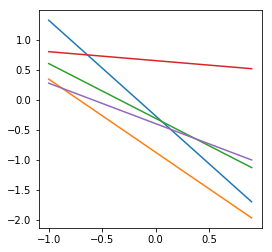
\includegraphics[width=\linewidth]{2-samples}
		\caption{Samples of $y$}
		\label{fig:2-s}
	\end{subfigure}
	\caption{Linear regression - 2 observations}
	\label{fig:2-s}
\end{figure}
\begin{figure}[H]
	\centering
	\begin{subfigure}[t]{0.3\linewidth}
		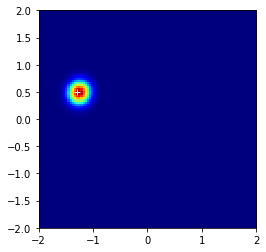
\includegraphics[width=\linewidth]{15-posterior}
		\caption{Posterior}
		\label{fig:15-p}
	\end{subfigure}
	\begin{subfigure}[t]{0.3\linewidth}
		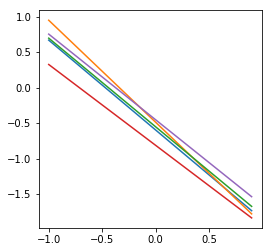
\includegraphics[width=\linewidth]{15-samples}
		\caption{Samples of $y$}
		\label{fig:15-s}
	\end{subfigure}
	\caption{Linear regression - 15 observations}
	\label{fig:15-s}
\end{figure} \\
\subsubsection{Non-parametric regression}
\question The covariance function, or kernel, encodes all the assumptions about the form of functions we are modelling, and often represents some form of “distance” or similarity between the data.

Figure \ref{fig:GP-p} shows samples from our GP-Prior created with a squared exponential covariance function. The length scale allows us to put constraints on how smooth the functions are. Small lengthscale values such as the one in Figure \ref{fig:0.1l} characterize functions that change quickly, whereas larger values such as the one in \ref{fig:10.l} characterize functions that change slowly.

The lengthscale therefore encodes our assumption of how smooth we think the underlying function will be.
\begin{figure}[H]
	\centering
	\begin{subfigure}[t]{0.3\linewidth}
		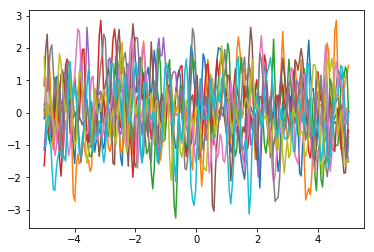
\includegraphics[width=\linewidth]{01}
		\caption{$\text{length scale} = 0.1$}
		\label{fig:0.1l}
	\end{subfigure}
	\begin{subfigure}[t]{0.3\linewidth}
		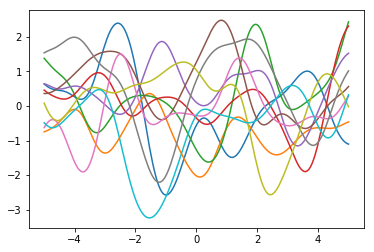
\includegraphics[width=\linewidth]{1}
		\caption{$\text{length scale} = 1.0$}
		\label{fig:1.0l}
	\end{subfigure}
	\begin{subfigure}[t]{0.3\linewidth}
		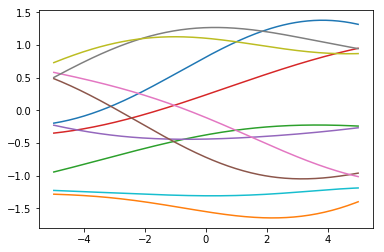
\includegraphics[width=\linewidth]{10}
		\caption{$\text{length scale} = 10$}
		\label{fig:10.l}
	\end{subfigure}
	\caption{GP-prior samples}
	\label{fig:GP-p}
\end{figure}
\question Figure \ref{fig:samples} shows the predictive posterior samples, our updated prior after having observed data. While our prior contained functions that corresponded to our general prior assumptions, the posterior shows only the set of constrained functions that pass by the observed data points.

We can observe from the samples in Figure \ref{fig:samples} and the variance in Figure \ref{fig:variance} (displayed as red shading at one standard deviation from the mean) that the uncertainty drops as we observe data but rises again as we move away from the observed data in the centre. This is due to our squared exponential covariance matrix that encodes our assumption that if two points $x_1$ and $x_2$ are close together, we expect their corresponding $y$ values to be close too. Therefore the further away a new $x$ value is from the $x$ values of observed data points the more uncertain we are about its $y$ value.

Adding a diagonal covariance matrix to the covariance function encodes a general uncertainty in our observations. This leads to a smoother function that approximates the data points rather than strictly interpolating between them. As we can see in Figure \ref{fig:variancewithdiag} this leads to a much larger standard deviation but a line that much closer approximates the underlying sine function.
\begin{figure}[H]
	\centering
	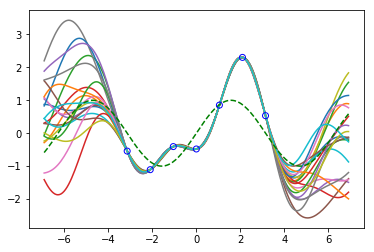
\includegraphics[width=0.4\linewidth]{samples}
	\caption{Predictive posterior samples}
	\label{fig:samples}
\end{figure}
\begin{figure}[H]
	\centering
	\begin{subfigure}[t]{0.4\linewidth}
		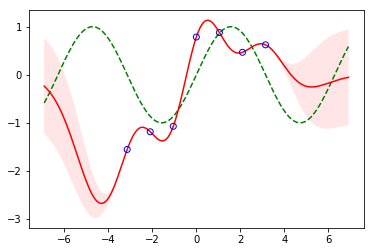
\includegraphics[width=\linewidth]{variance}
		\caption{Just kernel co-variance matrix}
		\label{fig:variance}
	\end{subfigure}
	\begin{subfigure}[t]{0.4\linewidth}
		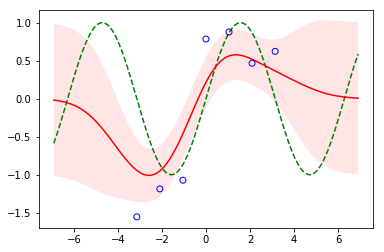
\includegraphics[width=\linewidth]{variancewithdiag}
		\caption{With diagonal co-variance matrix}
		\label{fig:variancewithdiag}
	\end{subfigure}
	\caption{Predictive mean and variances}
	\label{fig:muandcov}
\end{figure}
\section{The posterior}
\subsection{Theory}
\question Specifiying a prior assumption over $\mat{X}$ allows us to encode our preference about the nature of the properties that $\mat{X}$ should have. This assumption also constrains the variable $\mat{W}$ as $\mat{W}$ and $\mat{X}$ have a simple relationship.
\question We have encoded the assumption that all the dimensions in each variable of $\mat{X}$ are independent and identically distributed as we have used a Gaussian with an identity matrix as its covariance matrix.
\question We assume additive gaussian noise for a linear non-parametric Gaussian process and so our likelihood is as follows:
\begin{align*}
	p(y_i|x_i,\mat{W}) = \mathcal{N}(y_i|\mat{W}x_i, \sigma^2\mat{I})
\end{align*}
Our marginalisation is the product of two Gaussians which is itself another Gaussian.
\begin{align*}
	p(y_i|\mat{W}) &= \int p(y_i|x_i,\mat{W})p(x_i)\,dx \\
	&= \int \mathcal{N}(y_i|\mat{W}x_i, \sigma^2\mat{I})\,\mathcal{N}(0,\mat{I})\,dx
\end{align*}
By replacing these Gaussians with their probability density function and combining we can form a single exponential, by then completing the square with regard to $x$ we can integrate $x$ out to form a new exponent for the marginal which by re-arranging as we did in Question 6 we can find the mean $0$ and covariance $\mat{W}\mat{W}^T + \sigma^2\mat{I}$ thus making our marginal distribution:
\begin{align*}
	p(y_i|\mat{W}) = \mathcal{N}(y_i|0, \mat{W}\mat{W}^T + \sigma^2\mat{I})
\end{align*}
\subsubsection{Learning}
\question \emph{1.} The MAP estimate equals the mode of the posterior distribution while ML simply finds the parameters that maxmimise the likelihood. ML can be seen as a MAP that simply assumes a uniform prior distribution, or MAP can be seen as ML that employs a modified optimization objective by regularizing with the prior.

\emph{2.} As we observe more data the prior becomes less important relatively and the MAP estimate tends towards the ML estimate.

\emph{3.} We can ignore the denominator in Eq. 8 because the integral is with respect to $\mat{W}$ it is constant with respect to $\mat{W}$ and so has no bearing on the $\argmax_\mat{W}$.
\subsubsection{Practical optimisation}
\question \emph{1.} We have from Question 17 that:
\begin{align*}
	p(\mat{Y}|\mat{W}) = \prod_{i=1}^N\mathcal{N}(y_i|0,\mat{W}\mat{W}^T + \sigma^2\mat{I})
\end{align*}
then the objective function is derived as follows using log rules:
\begin{align*}
	\mathcal{L}(\mat{W}) &= -\log\bigg(\prod_{i=1}^N\mathcal{N}(y_i|0,\mat{W}\mat{W}^T + \sigma^2\mat{I})\bigg) \\
	&= -\sum_{i=1}^N\log\big(\mathcal{N}(y_i|0,\mat{W}\mat{W}^T + \sigma^2\mat{I})\big) \\
	&= -\sum_{i=1}^N\log\bigg(\frac{1}{\sqrt{2\pi\lvert\Sigma\rvert}}\bigg)+\log\bigg(\exp\Big(-\frac{1}{2}y_i^T\Sigma^{-1} y_i\Big)\bigg) \\
	&= -\sum_{i=1}^N\log\frac{1}{(2\pi)^{\frac{D}{2}}\lvert\mat{W}\mat{W}^T+\sigma^2\mat{I}\rvert^{\frac{1}{2}}}+\log\bigg(\exp\Big(-\frac{1}{2}y_i^T(\mat{W}\mat{W}^T+\sigma^2\mat{I})^{-1} y_i\Big)\bigg) \\
	&= -\log\big((2\pi)^D\lvert\mat{W}\mat{W}^T+\sigma^2\mat{I}\vert\big)^{-\frac{N}{2}} - \sum_{i=1}^N-\frac{1}{2}y_i^T(\mat{W}\mat{W}^T+\sigma^2\mat{I})^{-1} y_i \\
	&= \frac{N}{2}\bigg(D\log2\pi + \log(\lvert\mat{W}\mat{W}^T+\sigma^2\mat{I}\vert)\bigg) + \frac{1}{2}\sum_{i=1}^Ny_i^T(\mat{W}\mat{W}^T+\sigma^2\mat{I})^{-1} y_i
\end{align*}
From the fact that $\Tr(\mat{A}\mat{B}) = \Tr(\mat{B}\mat{A})$ and $\Tr(\mat{C} = \mat{c})$ for the dimensions in our sum we can evaluate it as follows:
\begin{align*}
	\mathcal{L}(\mat{W}) &= \frac{N}{2}\bigg(D\log2\pi + \log(\lvert\mat{W}\mat{W}^T+\sigma^2\mat{I}\vert) + \Tr\big((\mat{W}\mat{W}^T+\sigma^2\mat{I})^{-1}\mat{Y}\mat{Y}^T\big)\bigg)
\end{align*}
\emph{2.} To find the gradient of $\mathcal{L}$ we will look at each term in turn:
\begin{align*}
	\mathcal{L}(\mat{W}) &= \frac{N}{2}\bigg(\overbrace{\Tr\big((\mat{W}\mat{W}^T+\sigma^2\mat{I})^{-1}\mat{Y}\mat{Y}^T\big)}^{A} + \overbrace{\log(\lvert\mat{W}\mat{W}^T+\sigma^2\mat{I}\vert)}^{B} + \overbrace{D\log2\pi}^{C}\bigg)
\end{align*}
$C$ is a constant term so we shall discard that. To find the derivative of $B$ we use the rules that $\partial(\log(\det(\mat{X}))) = \Tr(\mat{X}^{-1}\partial\mat{X})$ and that $\sigma^2\mat{I}$ is constant with respect to $\mat{W}$ and so evaluate $B$ to:
\begin{align*}
	\frac{\partial B}{\partial\mat{W}} &= \Tr\Big((\mat{W}\mat{W}^T+\sigma^2\mat{I})^{-1}\partial(\mat{W}\mat{W}^T)\Big)
\end{align*}
We also have the rules that $\partial(\mat{X}\mat{Y}) = (\partial\mat{X})\mat{Y} + \mat{X}(\partial\mat{Y})$ and that $\frac{\partial\mat{X}}{\partial\mat{X}_{ij}} = \mat{J}^{ij}$ where $\mat{J}$ is the single-entry matrix, having $1$ at $(i, j)$ and $0$ elsewhere and so can reduce $B$ to:
\begin{align*}
	\frac{\partial B}{\partial\mat{W}_{ij}} &= \Tr\Big((\mat{W}\mat{W}^T+\sigma^2\mat{I})^{-1}(\mat{J}^{ij}\mat{W}^T + \mat{W}\mat{J}^{ij}^T)\Big)
\end{align*}
Using the earlier rules along with the rule that $\partial(\Tr(\mat{X}))=\Tr(\partial\mat{X})$ we can find the derivative of $A$:
\begin{align*}
	\frac{\partial A}{\partial\mat{W}} &= \Tr\bigg(\partial\Big(\mat{Y}(\mat{W}\mat{W}^T+\sigma^2\mat{I})^{-1}\mat{Y}^T\Big)\bigg) \\
	&= \Tr\Bigg(\mat{Y}\mat{Y}^T\partial\Big((\mat{W}\mat{W}^T+\sigma^2\mat{I})^{-1}\Big) + (\mat{W}\mat{W}^T+\sigma^2\mat{I})^{-1}\Big(\partial(\mat{Y}^T\mat{Y})\Big)\bigg)
\end{align*}
As $\partial(\mat{X}^{-1}) = -\mat{X}^{-1}(\partial\mat{X})\mat{X}^{-1}$ we can reduce $A$ to:
\begin{align*}
	\frac{\partial A}{\partial\mat{W}} &= \Tr\Bigg(\mat{Y}\mat{Y}^T\partial\Big((\mat{W}\mat{W}^T+\sigma^2\mat{I})^{-1}\Big)\Bigg) \\
	\frac{\partial B}{\partial\mat{W}_{ij}} &= \Tr\Bigg(\mat{Y}\mat{Y}^T\Big(-(\mat{W}\mat{W}^T+\sigma^2\mat{I})^{-1}(\mat{J}^{ij}\mat{W}^T + \mat{W}\mat{J}^{ij}^T)(\mat{W}\mat{W}^T+\sigma^2\mat{I})\Big)\Bigg)
\end{align*}
And so by combining our terms $A$ and $B$ we have the gradient for our log likelihood $\mathcal{L}$:
\begin{align*}
	\frac{\partial\mathcal{L}}{\partial\mat{W}_{ij}} =\ &\frac{N}{2}\Tr\Bigg(\mat{Y}\Big(-(\mat{W}\mat{W}^T+\sigma^2\mat{I})^{-1}(\mat{J}^{ij}\mat{W}^T + \mat{W}\mat{J}^{ij}^T)(\mat{W}\mat{W}^T+\sigma^2\mat{I})\Big)\mat{Y}^T\Bigg) \\
	&+ \frac{N}{2}\Tr\Big((\mat{W}\mat{W}^T+\sigma^2\mat{I})^{-1}(\mat{J}^{ij}\mat{W}^T + \mat{W}\mat{J}^{ij}^T)\Big)
\end{align*}
\subsubsection{Non-parametric}
\question [TODO]
\subsection{Practical}
\subsubsection{Linear representation learning}
\question We minimised the objective function to get our maximum likelihood estimate for $\mat{W}$
\begin{align*}
	\mat{W}^\prime = \argmin_\mat{W} \mathcal{L}(\mat{W})
\end{align*}
To find the representation for $\mat{X}^\prime$ we must know the reverse of the linear mapping.
\begin{align*}
	\mat{Y} &= \mat{X}^\prime\mat{W}^\prime^T \\
	\mat{X}^\prime &= \mat{Y}\mat{W}^\prime(\mat{W}^\prime^T\mat{W}^\prime)^{-1}
\end{align*}
And then use minimization of our objective function using the non-linear conjugate gradient method to find $\mat{X}^\prime$.
\begin{figure}[H]
	\centering
	\begin{subfigure}[t]{0.4\linewidth}
		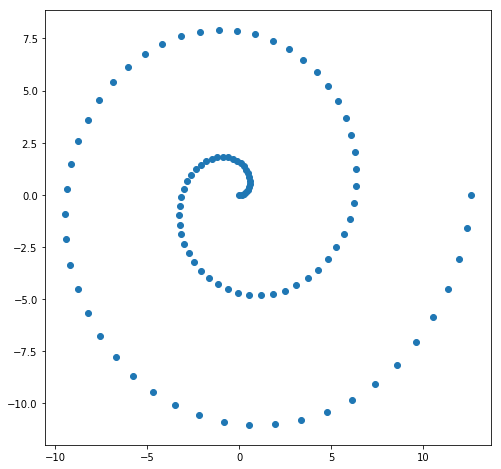
\includegraphics[width=\linewidth]{oldX}
		\caption{Original $\mat{X}^\prime$}
		\label{fig:oldX}
	\end{subfigure}
	\begin{subfigure}[t]{0.4\linewidth}
		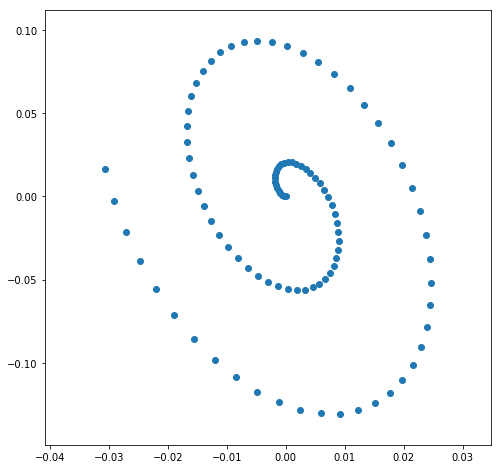
\includegraphics[width=\linewidth]{newX}
		\caption{Learned $\mat{X}^\prime$}
		\label{fig:newX}
	\end{subfigure}
	\caption{Representation Learning of $\mat{X}^\prime$}
\end{figure}
Our learned representation of $\mat{X}^\prime$ is very close to the correct shape only rotated slightly, this is because the marginal likelihood we are maximising is invariant to any matrix transformation whose inverse is its own transposition i.e. any matrix for which $\mat{R}\mat{R}^T = \mat{I}$ (rotations along with a few other transformations fall into this category). Therefore any of these transformations can be applied to $\mat{W}$ without the marginal likelihood changing. We can see this by setting $\mat{W}$ in the likelihood to $\mat{W}^\prime\mat{R}$:
\begin{align*}
	\mathcal{L}(\mat{W}) &= -\sum_{i=1}^N\log\big(\mathcal{N}(y_i|0,(\mat{W}^\prime\mat{R})(\mat{W}^\prime\mat{R})^T + \sigma^2\mat{I})\big) \\
	&= -\sum_{i=1}^N\log\big(\mathcal{N}(y_i|0,\mat{W}^\prime\mat{R}\mat{R}^T\mat{W}^\prime^T + \sigma^2\mat{I})\big) \\
	&= -\sum_{i=1}^N\log\big(\mathcal{N}(y_i|0,\mat{W}^\prime\mat{W}^\prime^T + \sigma^2\mat{I})\big)
\end{align*}
\end{document}
